% !TeX spellcheck = en_US
% Time-stamp: <09/10/02 01:57:13 vilhuber>
% $Id: Presentation-PSD2014-SynBDS.tex 1720 2015-09-25 14:29:12Z lv39 $

% normal line:
\documentclass[xcolor=table,compress]{beamer}
% to create notes:
%\documentclass[handout,notes=only]{beamer}
% to create handouts
%\documentclass[xcolor=table,handout,compress]{beamer}
% to create a different kind of handouts
%\documentclass{article}
%\usepackage[envcountsect]{beamerarticle}

%\setbeameroption{handout}
%\setbeameroption{show notes}


%
% Packages
%
\mode<article> % only for the article version
{
  \usepackage{fullpage}
  \usepackage{hyperref}
}

\usepackage{ifpdf}
\ifpdf
\usepackage{embedfile}
\embedfile{\jobname.tex}
\fi

\usepackage{graphicx}
%\usepackage{pstricks}
\usepackage{xcolor}
\usepackage{pifont}
%\usepackage{../chicago}
\usepackage{pgf}
\usepackage{amsmath,amssymb,amsfonts}
\usepackage[latin1]{inputenc}
\usepackage{colortbl}
\usepackage[english]{babel}
\usepackage{array}
\usepackage{pdfpages}

\usepackage{csvsimple}
\usepackage{tikz}
\usepackage{calc}
\usepackage{algpseudocode}
\newenvironment{algorithm}{\begin{center}\hrule\ \\}{\hrule\end{center}}
\usepackage[printonlyused]{acronym}

% usage:
%   \includepdf[pages={1}]{myfile.pdf}
%   \includepdf[pages={1,3,5}]{myfile.pdf} would include pages 1, 3, and 5 of the file. 
%   To include the entire file, you specify pages={-}, where {-}
%\usepackage{landscape}

%\usepackage{lmodern}
%\usepackage[T1]{fontenc}

\usepackage{times}
%\usepackage{colortbl}

%============================================================
% Beamer specific styles and configs
%============================================================

\mode<presentation>
{
% alternative, could always use
%\usetheme{Census}
\usetheme{cornell}
\useoutertheme{cornell}


% For Census template
%\usetheme{Malmoe}
%\usecolortheme{dove}
%\setbeamertemplate{background canvas}{\includegraphics
%        [height=\paperheight]{Census2014-background-4x3}}
%\setbeamertemplate{footline}[frame number]% page numbers and using Warsaw theme%
%\setbeamertemplate{navigation symbols}{}
}
%\setbeamercovered{dynamic}


%============================================================
% Title
%============================================================

\title[SynBDS]{Using partially synthetic data to replace suppression in the Business 
Dynamics Statistics: early results}
\author[Miranda, Vilhuber]{%
Javier Miranda\inst{2}%
\and %
  Lars~Vilhuber\inst{1} 
}

\institute[Cornell]{
  \inst{1}%
   Labor Dynamics Institute,
  ILR, Cornell University, United States
\and \inst{2} Center for Economic Studies, U.S. Census Bureau, United States
}%
\date[September 2014]{September 2014, PSD2014, Eivissa }
\subject{Synthetic Data; Establishment Microdata}

%
% Some useful commands
%

\newcommand{\rarrow}{\selectfont\ding{220}}
\newcommand{\skiplink}{\tiny{\gray\selectfont\ding{59}}}
\newcommand{\goback}{\Acrobatmenu{GoBack}{\gray\selectfont\ding{242}}}
\newcommand{\x}{\selectfont\ding{52}}
\newcommand{\verbatimsize}{\tiny}
\newcommand{\tablesize}{\footnotesize}

%
% The document proper
%
\begin{document}

\frame{\titlepage}

%\part<presentation>*{Outline}
%
%\begin{frame}
%  \frametitle{Outline}
%  \tableofcontents[part=1,pausesections]
%\end{frame}

% This puts the partial table of contents at the start of each subsection
%\AtBeginSubsection[]
%{
%  \begin{frame}<beamer>
%    \frametitle{Outline}
%    \tableofcontents[current,currentsubsection]
%  \end{frame}
%}

\part<presentation>{Main Talk}

%
%  From this point on, we should probably extract it to a sub-document
%

%TCIDATA{Version=5.00.0.2570}
%TCIDATA{LaTeXparent=0,0,Presentation-CAFE-displacement-subdoc.tex}
% $Id: Presentation-subdoc.tex 1720 2015-09-25 14:29:12Z lv39 $
% $URL: https://forge.cornell.edu/svn/repos/ncrn-cornell/branches/papers/PSD2014/text/Presentation/Presentation-subdoc.tex $
\section{Context}
\begin{frame}
\begin{block}{Funding}
\begin{itemize}
\item Vilhuber's work is partially funded by NSF Grant \href{http://www.nsf.gov/awardsearch/showAward.do?AwardNumber=1042181}{\#1042181}. 
\end{itemize}
\end{block}
\begin{block}{Disclaimer}
This paper reports the results of research and analysis 
undertaken by Census Bureau staff. It has undergone a more limited review by the Census Bureau than its 
official publications. This report is released to inform interested parties and to encourage discussion. Any 
findings, conclusions or opinions are those of the authors. They do not necessarily reflect those of the Center for 
Economic Studies, the U.S. Census Bureau, or the National Science Foundation. 
\end{block}
\end{frame}


\begin{frame}
\begin{block}{Business Dynamics}
"The U.S. economy is comprised of over 6 million establishments with paid employees. The population of these businesses is constantly churning -- some businesses grow, others decline and yet others close. New businesses are constantly replenishing this pool."[\href{https://www.census.gov/ces/dataproducts/bds/overview.html}{*}]
\end{block}
\begin{block}{Questions}
\begin{itemize}
\item Small businesses' contribution to job and productivity growth 
\item ... or is it \alert{young} businesses' contribution?
\item Dynamics of businesses in their early (post-founding) years
\end{itemize}
\end{block}
\end{frame}

\begin{frame}{Data for Business Statistics in the United States}
\begin{block}{Provided by the US Census Bureau}
\begin{itemize}
\item County Business Patterns (CBP)
\item Annual Survey of Manufactures (ASM)
\item and over 100 separate additional surveys..
\item Economic Census
\item Business Dynamic Statistics (BDS)
\item Quarterly Workforce Indicators (QWI)
\end{itemize}
\end{block}
\pause
\begin{block}{Provided by others}
\begin{itemize}
\item Quarterly Census of Employment and Wages (QCEW, by BLS)
\item Compustat (S \& P)
\end{itemize}
\end{block}
\end{frame}

\begin{frame}{Business Microdata at the Census Bureau}
\begin{center}
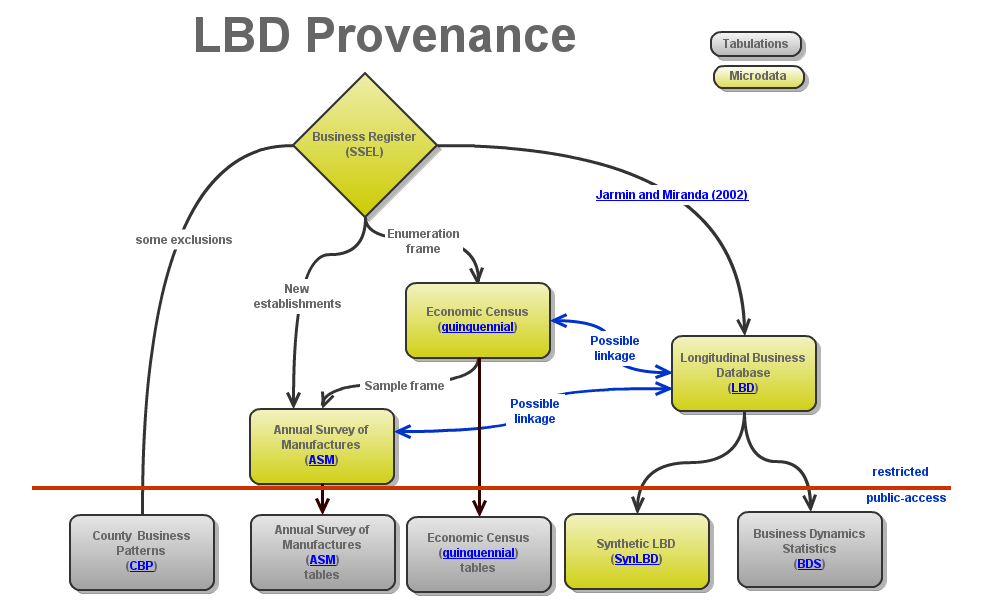
\includegraphics[height=0.8\textheight]{./LBD_Provenance_v2}
\end{center}
\end{frame}

\begin{frame}{Business Microdata at the Census Bureau}
\only<1>{
\begin{center}
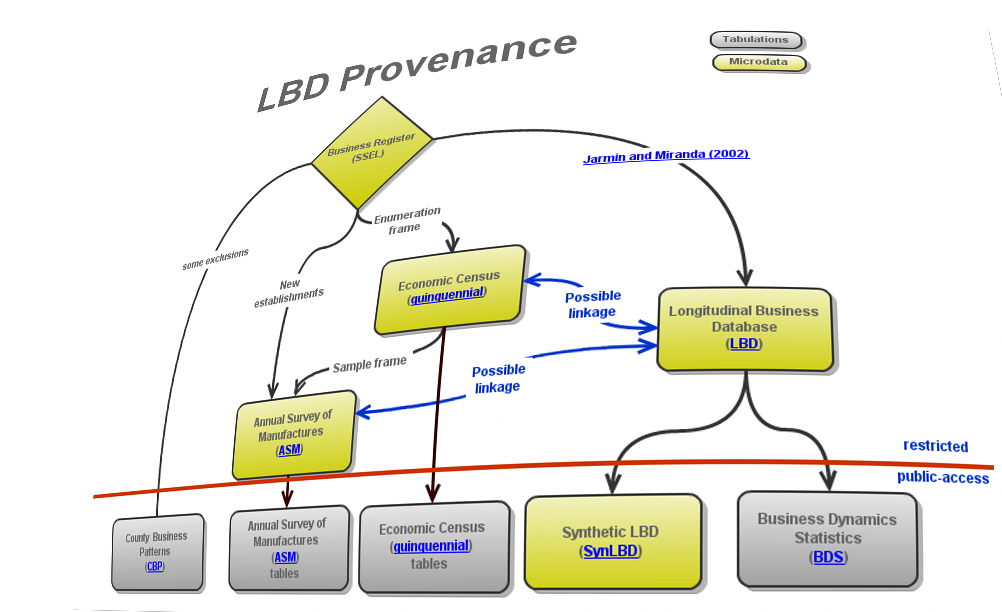
\includegraphics[height=0.8\textheight]{./LBD_Provenance_v2_tilted}
\end{center}}
\pause
\only<2>{
\begin{center}
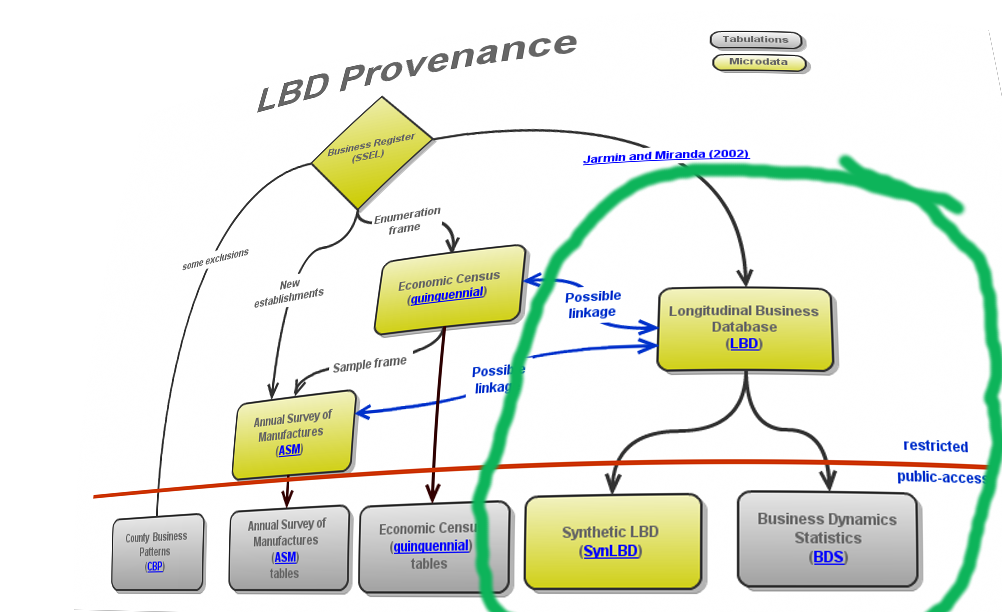
\includegraphics[height=0.8\textheight]{./LBD_Provenance_v2_tilted_hilite}
\end{center}}
\end{frame}



\begin{frame}{Business Dynamic Statistics}
\begin{block}{Annual data series}
\begin{itemize}
\item Establishment - level business dynamics: by firm age and firm size
\item Employment - job creation and destruction
\item Job expansions and contractions
\item Number of establishments
\item Establishment openings and closings
\item Number of startups and firm shutdowns   
\end{itemize}
\end{block}
More info: \href{http://www.census.gov/ces/dataproducts/bds/}{www.census.gov/ces/dataproducts/bds/}
\end{frame}

\begin{frame}{Available BDS tabulations}
\begin{block}{Firm and Establishment Characteristics}
\begin{itemize}
\item Sector
\item Firm Size
\item Firm Age
\item Initial Firm Size
\item Geography (State, Metro/Non-metro, MSA)
\item Cross-tabulations by up to three of these characteristics
\end{itemize}
\end{block}
\begin{block}{Lots of detail}
62 very detailed tables
\end{block}
\end{frame}

\begin{frame}{Disclosure avoidance in the BDS}
\begin{block}{P-percent rule with secondary suppressions}
\begin{itemize}[<+->]
\item Cells where the top 2 firms account for more than \emph{P} percent of the total value of the cell are flagged for suppression
\item \emph{P} value is not disclosed
\item Trivially: cells with fewer than 3 firms represented are always suppressed
\item Secondary suppressions: ``minimize the amount of information loss in a given table row or column''.
\end{itemize}
\end{block}
\end{frame}


\begin{frame}{Extent of suppression}
%\csvautotabular{programs/bds_e_suppressions_multi.csv}
\tiny
\begin{table}
\caption{Suppressions in establishment-level BDS\label{tab:bds_e}}
\centering
\begin{tabular}{|lc|r|rr|}\hline%
               &                 &\bfseries Number &\multicolumn{2}{c|}{\bfseries Suppressions (\%)}\\
\cline{4-5}
\bfseries Type & \bfseries Level &\bfseries of     &                            & \bfseries Job creation\\
                            &                              &\bfseries  cells& \bfseries Any  &\bfseries by entrants\\
\hline
\csvreader[head to column names,late after line=\\,late after last line=\\\hline]%
{../programs/bds_e_suppressions_multi.csv}{}%
{\typename & \level & \cells & \percentsup  & \jcbirths}%
\multicolumn{5}{p{0.6\textwidth}}{\footnotesize Note: Cells are year $x$ categories, where the 
number of categories varies by published table.}
\end{tabular}
\end{table}
\end{frame}

\begin{frame}{Extent of suppression}
\begin{center}
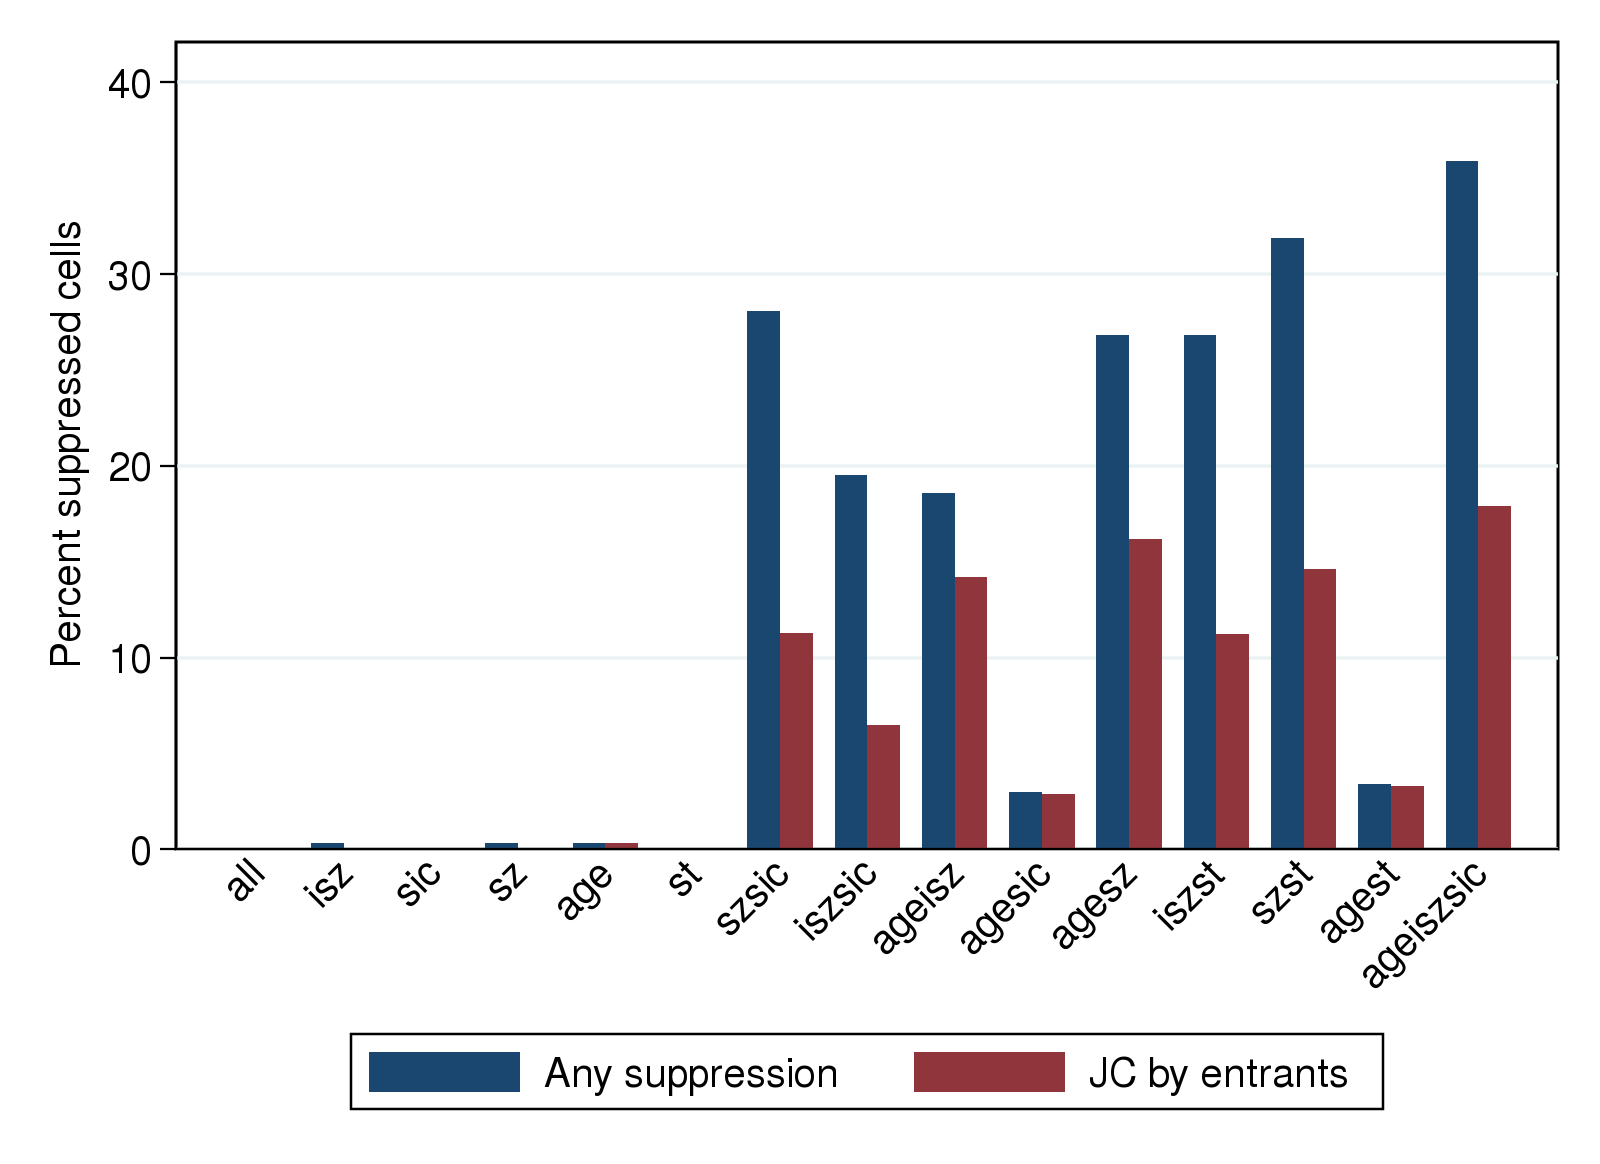
\includegraphics[height=0.8\textheight]{./suppressions_estabs}
\end{center}
\end{frame}

\section[Solution]{Proposed solution}

\begin{frame}{Business Microdata at the Census Bureau}
\begin{center}
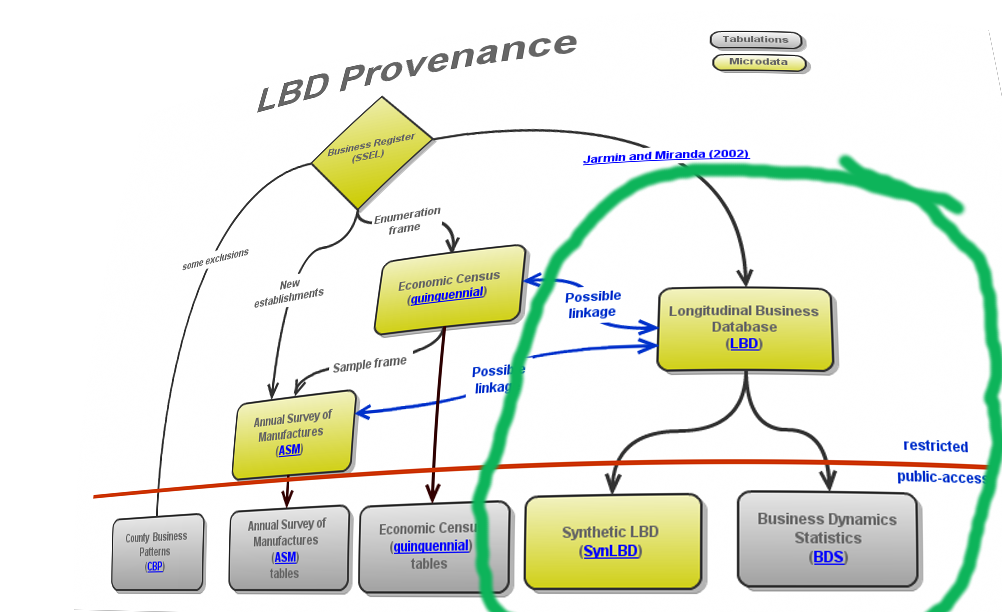
\includegraphics[height=0.8\textheight]{./LBD_Provenance_v2_tilted_hilite}
\end{center}
\end{frame}


\begin{frame}{Purpose of SynLBD}
\begin{block}{The SynLBD is }
\begin{itemize}[<+->]
\item derived from confidential Longitudinal Business Database (LBD, \cite{MirandaJarmin2002})
\item designed to facilitate researcher access to establishment microdata (LBD)
\item while preserving the confidentiality of establishment/business data. 
\item part of a larger strategy by the Census Bureau to provide \textit{better 
statistics on business dynamics} CNSTAT  \cite{CNSTATBusinessDynamics}
\end{itemize}
\end{block}
\end{frame}


\begin{frame}{Contents of (Syn)LBD}
\begin{block}{Data elements}
\begin{itemize}
\item  longitudinal establishment identifiers (created using probabilistic matching \cite{MirandaJarmin2002}) \onslide<2->{\alert{Masked}}
\item information on birth, death \onslide<2->{\alert{Synthesized}}
\item  employment and payroll over time \onslide<2->{\alert{Synthesized}}
\item location \onslide<2->{\alert{Suppressed}}
\item industry \onslide<2->{\alert{Released}}
\item firm  affiliation of  employer establishments \onslide<2->{\alert{$\rightarrow$ next version}}
\end{itemize}
\end{block}
\pause
\pause
\begin{block}{Complete description}
Kinney et al \cite{KinneyEtAl2011}
\end{block}
\tiny \hfill[\hyperref[sec:SynLBD_details]{more}]
\end{frame}

\begin{frame}
\begin{block}{Putting two and two together...}
\begin{itemize}[<+->]
\item[] 
V2.0 of SynLBD released by Census Bureau's Disclosure Review Board in 2011
\item[]
Let's combine public-use data to fill in suppressions

\end{itemize}
\end{block}
\end{frame}


\begin{frame}{Combining synthetic and protected data}
\begin{block}{Initially...}
\begin{itemize}
\item[...] explored as part of \href{http://www.myweb.ttu.edu/rgitting/}{Kaj Gitting}'s thesis \cite{Gittings2009thesis}
\item[...] expanded as part of our FCSM paper \cite{AbowdEtAl2012}
\end{itemize}
\end{block}
\begin{block}{Could it work for BDS?}
\begin{itemize}
\item LBD underlies BDS
\item SynLBD derived from LBD
\item SynLBD proven analytic validity
\end{itemize}
\end{block}
\end{frame}

\begin{frame}{Analytic validity}
\begin{center}
\only<1>{
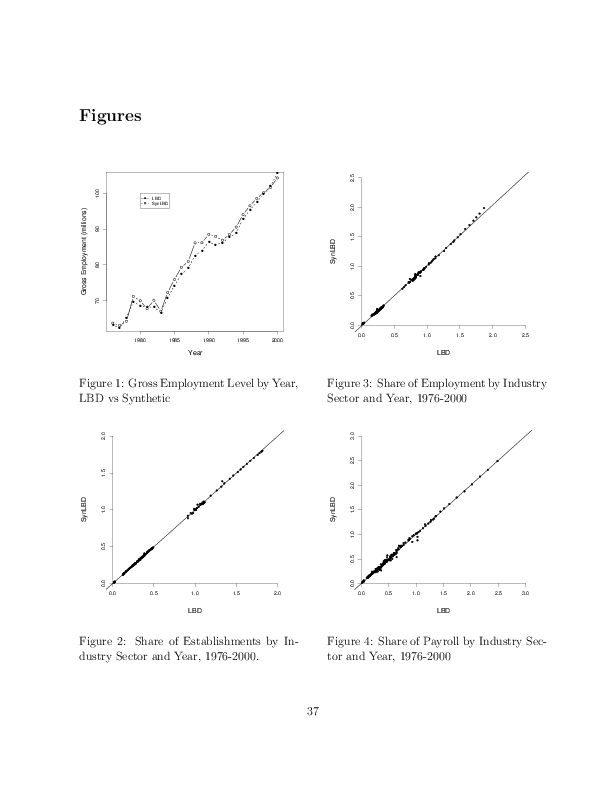
\includegraphics[height=0.8\textheight]{./CES-WP-11-04-page37}
}
\only<2>{
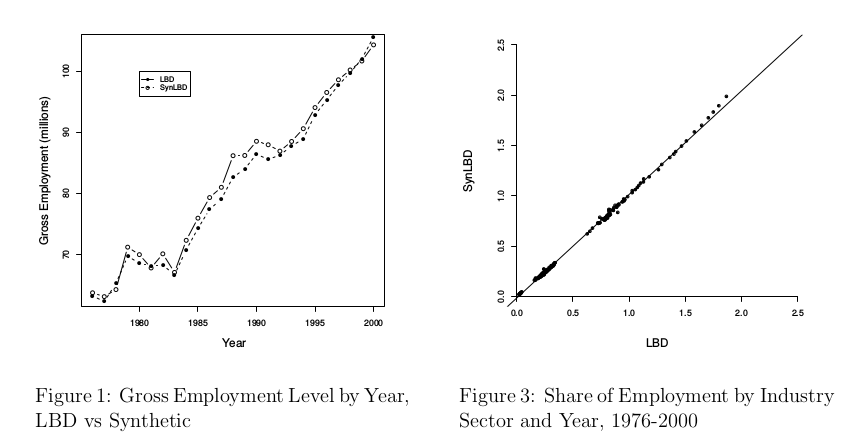
\includegraphics[width=\textwidth]{./CES-WP-11-04-page37-hilite}
}
\end{center}
\end{frame}

\begin{frame}{Analytic validity}
\begin{center}
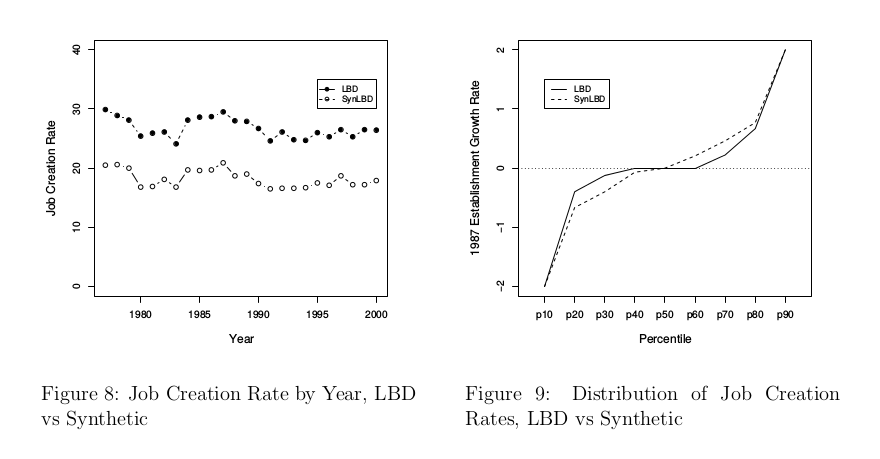
\includegraphics[width=\textwidth]{./CES-WP-11-04-page39-hilite}
\end{center}
\end{frame}




\begin{frame}{Notation}

\begin{block}{Base variable}
Establishment employment $e_{jt}$. 
\end{block}
\begin{block}{Example}
\begin{eqnarray}
\label{eq:e_birth}
birth_{jt} &=& \left \lbrace 
\begin{array}{rl}
1 &\mbox{if}~~  e_{jt} > 0 ~~ \mbox{and}  ~~e_{jt-s} = 0 ~~\forall s\geq 1~~\\
0 &\mbox{otherwise}
\end{array} \right .
\end{eqnarray}
\begin{eqnarray}
\label{eq:e_birth}
jcbirth_{jt} &=& \left \lbrace 
\begin{array}{rl}
e_{jt}-e{jt-1} &\mbox{if}~~  e_{jt} > 0 ~~ \mbox{and}  ~~e_{jt-s} = 0 ~~\forall s\geq 1~~\\
0 &\mbox{otherwise}
\end{array} \right .
\end{eqnarray}
\end{block}
\end{frame}

\begin{frame}{Notation}
\begin{block}{Synthetic values}
Synthesized version of variable $x_{jt}$ is 
denoted $\tilde{x}_jt$. 
\end{block}
\begin{block}{Cells}
\begin{itemize}
\item[]
Collections of characteristics $k_t(j)$ (industry, geography, establishment or firm age and size)
\item[]  $j \in 
K_t^\prime$ describes the set of firms at time $t$ such that $k_t(j)=k^\prime$.  

\end{itemize}
\end{block}
\end{frame}

\begin{frame}{Notation}
\begin{block}{Aggregations}
Generically in capital letters:
\begin{equation}
\label{eq:national_e}
E_{\cdot t} = \sum_{i=1}^J e_{it},
\end{equation}

Aggregations across establishments having characteristics $k^\prime$ at 
time $t$
\begin{equation}
\label{eq:sum_X}
X_{k^\prime t} =  \sum_{j \in K_t^\prime} x_{jt}
\end{equation}
\end{block}
\end{frame}

\begin{frame}{Suppression rules }
\begin{block}{Suppression rules}
for (aggregate) variable $X$ are captured by $I_{t}^X$, such that the 
releasable variable $X^o$  under the current regime can be described by

\begin{eqnarray}
\label{eq:supp_x}
X_{k^\prime t}^o &=& \left \lbrace 
\begin{array}{rl}
X_{k^\prime t} &\mbox{if}~~  I_{kt}^X = 1 \\
\mbox{missing} &\mbox{otherwise}
\end{array} \right .
\end{eqnarray}
\end{block}
\end{frame}



\subsection{Algorithm 1: Drop-in}
\begin{frame}[fragile]{Algorithm 1}

We can now express the ``drop-in'' algorithm, leading to the released variable $X^{(i)}$, as:
\begin{block}{BDS$^{(i)}$}
\begin{algorithm}
\begin{algorithmic}
\If {$I_{t}^X = 1$ }
    \State {$X_{k^\prime t}^{(i)} = X_{k^\prime t} $}
\Else
        \State {$X_{k^\prime t}^{(i)} =\tilde{X}_{k^\prime t} $}
\EndIf
\end{algorithmic}
\end{algorithm}
\end{block}
\end{frame}

%\begin{note}
%Thus, simply computing a ``SynBDS'', based on the \ac{SynLBD}, in parallel to the 
%computation 
%of the \ac{BDS} (based on the confidential \ac{LBD}), and replacing suppressed cells with their 
%fully synthetic counterparts, yields a dataset without missing observations. Variations can 
%encompass using the average of multiple implicates  as the replacement value. In 
%general, increasing the number of implicates will improve the analytic validity, but reduce the 
%protection provided by the synthesis process. 
%
%Because no time-consistency is imposed, this method can lead to seam biases or higher 
%intertemporal variance. We will return to this issue in Section~\ref{sec:analysis}. For later 
%reference, we denote the tabulations created by Algorithm~1 as \textbf{BDS$^{(i)}$}.
%\end{note}


\section[Results]{Early results}


\begin{frame}{Analysis}
\begin{block}{Analysis}
\begin{itemize}[<+->]
\item We implemented Algorithm~1 for \ac{BDS} tabulations by \alert{establishment age and 
size} ({\tt bds\_e\_agesz}). 
\item About 26\% of all cells have some suppression
\item Here: variable, ``Job Creation by establishment births'' ({\tt job\_creation\_births}). 
\end{itemize}
\end{block}
\end{frame}

\subsection{Protection}
\begin{frame}{Protection}
\begin{block}{Protection through synthesis}
\begin{itemize}[<+->]
\item Cells are filled in with data available to a wide audience (public-use)
\item ....(but which typically cannot create tabulations)
\item ....(future tables will contain variables which are not currently available on the synthetic 
data file)
\item Structurally: the synthetic data are ... fully synthetic (discussed in Kinney et al, 2011)
\item Additional comparison: differences in each cell
\end{itemize}
\end{block}
\end{frame}


\begin{frame}{From Kinney et al}
\begin{columns}
\begin{column}{0.6\textwidth}
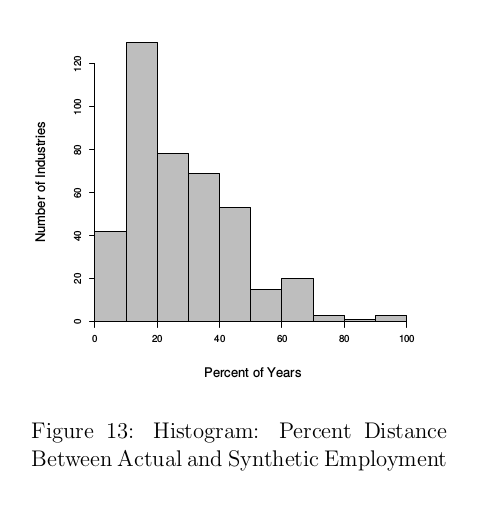
\includegraphics[height=0.8\textheight]{CES-WP-11-04-page40-figure13}
\end{column}
\begin{column}{0.3\textwidth}
The comparison is for individual establishments, not within cells
\end{column}
\end{columns}
\end{frame}

\begin{frame}{Cell-wise comparison}
\begin{block}{Criteria for cell-wise comparison}
\begin{itemize}
\item Differences in count of establishment in a cell
\item Differences in values of cells
\end{itemize}
\end{block}
Not done yet.
\end{frame}


\subsection{Analytic validity}

\begin{frame}{Analytic validity: time-series}
\begin{block}{Setup}
Estimate an AR(2) process for each of 
$X_{k^\prime t}$, $X_{k^\prime t}^{s}$, and $X_{k^\prime t}^{(i)}$
\end{block}
\begin{block}{Metrics}
\begin{itemize}
\item  number of missing time-series estimates %(repeated suppressions in $X_{k^\prime t}^{s}$ 
%may lead to time-series that are too short),
\item the number of significant coefficients for the first lag of the AR(2)
\item \emph{coverage}, the 
percentage of regressions where the true $\rho_1$ lies within the confidence band around the 
coefficient estimated from the comparison $\rho_1^{s}$ and $\rho_1^{(i)}$, 
\item interval overlap measure $J_k$ \cite{tas2006}
\end{itemize}
\end{block}
\end{frame}


\begin{frame}[fragile]{Analytic validity}
\begin{center}
%\small
%\begin{table}
%\caption{Analytic validity of published data\label{tab:bds_e_pub2}}
%\centering
%%\begin{tabular}{|lc|r|rrr|}\hline%
%\csvreader[tabular=|l|r|rr|rrr|rr|rr|,table head=\hline 
%	&Number 
%	&\multicolumn{2}{c|}{} 
%	& \multicolumn{3}{c|}{Percent} 
%	&\multicolumn{2}{c|}{}
%	&\multicolumn{2}{c|}{Interval}\\
%Variable 
%	&feasible 
%	& \multicolumn{2}{c|}{Missing}                
%	& \multicolumn{3}{c|}{significant}
%	&\multicolumn{2}{c|}{Coverage}
%	&\multicolumn{2}{c|}{overlap}\\
%    & $X_{k^\prime t}^{}$ 
%    & $X_{k^\prime t}^{s}$ & $X_{k^\prime t}^{(i)}$
%    & $\rho_1$ & $\rho_1^{s}$&$\rho_1^{(i)}$
%    & $\rho_1^{s}$&$\rho_1^{(i)}$
%    & $J_1^{s}$&$J_1^{(i)}$
%    \\\hline,
%	late after line=\\,late after last line=\\\hline]%
%{../programs/r_e_agesz_all_combined_mod.csv}{Variable=\V,Jk=\Jk,Jks=\Jks,coverage=\mycr,coverages=\mycs,missing=\mr,missings=\m2,significanti2=\si,number=\N,significantr2=\sr,significant22=\s2}%
%{\V & \N & \mr & \m2 & \si &\sr & \s2 &\mycr & \mycs & \Jk & \Jks}%
%
%\end{table}


%% Alternatively:
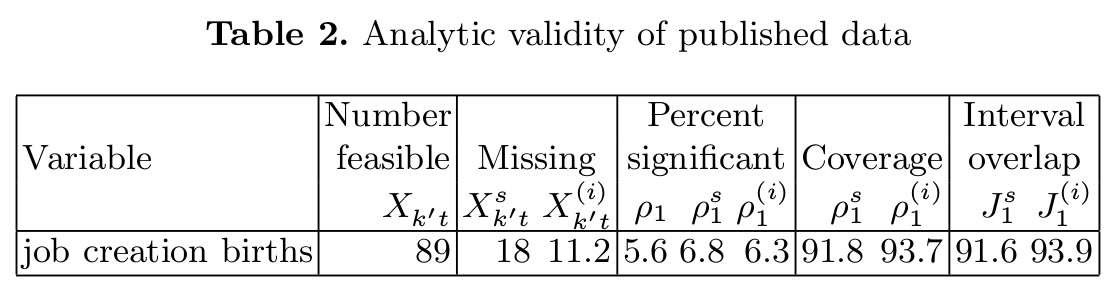
\includegraphics[width=\textwidth]{table2}

\end{center}
\end{frame}

%\begin{frame}{Notation}
%\begin{block}{Aggregations}
%E.g. national employment 
%\begin{equation}
%\label{eq:national_e}
%E_{\cdot t} = \sum_{i=1}^J e_{it},
%\end{equation}
%(national) establishment births are
%\begin{equation}
%\label{eq:national_birth}
%Birth_{\cdot t} = \sum_{i=1}^J birth_{it},
%\end{equation}
%and job creation by births
%\begin{equation}
%\label{eq:national_jcbirth}
%JCBirth_{\cdot t} = \sum_{i=1}^J jcbirth_{it},
%\end{equation}
%
%\end{block}
%\end{frame}

















\section{Conclusion}

\begin{frame}{Open issues}
\begin{block}{Unexplored issues}
\begin{itemize}[<+->]
\item SynLBD is synthesized independently within industry
\item Geography is not synthesized, not considered within synthesis process (and not released) 
- unclear how geography subtabulations will fare, what the disclosure avoidance implications are
\item Firm-level characteristics go into a bit more detail, and require availability of SynLBD v3
\item Time consistency of the series
\item Comparison to alternative ``outside-the-firewall'' imputation mechanisms 
(\cite{HolanEtAl2010,BradleyEtAl2014})
\end{itemize}
\end{block}
\end{frame}

\begin{frame}[fragile]{Postulated alternative algorithm}
%In part to address the possible time-inconsistencies we propose an 
%alternative algorithm.  In order to minimize future seam issues, we remove establishments (or 
%firms) that 
%contribute to sensitive cells of tabulations with characteristics $k^\prime t$, for $t$ and the 
%next 
%$n$ periods. These establishments are replaced by  synthetic establishments that match on 
%characteristics $k^\prime t$, and we simply replace the observed values in the database 
%$x_{js}$ 
%with the synthetic values $\tilde{x}_{js}$ (for all variables), for $s=t,\dots,t+n$.%
%\footnote{We thus re-use the index $j$ for both observed and synthetic establishments.}
%For convenience, denote by $J_{k^\prime t}^-$ the set of establishments for which observed 
%values $x_{jt}$ do not contribute to any tabulations at time $t$.  In its simplest form, the 
%algorithm can be expressed as
\begin{block}{$BDS^{(ii)}$}
\begin{algorithm}
\begin{algorithmic}
\State {Compute: $X_{k^\prime t} = \sum_{j \in K_t^\prime} x_{jt}$}
\State{Compute: $I_{t}^X$}
\If {$I_{t}^X = 0$ }
    \State {Assign all $j \in K_t^\prime$ to $J_{k^\prime t}^-$ }
    \State {Assign all $j \in J_{k^\prime s}^-$ to $J_{k^\prime t}^-$ for $t > s > t-n$}
\EndIf
\State { Compute: %
$$X_{k^\prime t}^{(ii)} = 
               \sum_{j \in \left \lbrace K_t^\prime \cap J_{k^\prime t}^- \right \rbrace }
                               \tilde{x}_{jt} 
	          +
	          \sum_{j \in  K_t^\prime \wedge j \notin J_{k^\prime t}^-  }
	                                         {x}_{jt} 
$$}

\end{algorithmic}
\end{algorithm}

For $n=\infty$, $J_{t}$ is an absorbing set, which seems undesirable. For $n=1$, this reduces  to 
Algorithm~1.
\end{block}
\end{frame}




\begin{frame}{Conclusion}
\begin{block}{Early in the process}
\begin{itemize}
\item Desirable a-priori properties (use of public-use data to fill in blanks)
\item May not work for other variables
\item Assumes suppression as primary disclosure avoidance mechanism...
\end{itemize}\end{block}
\end{frame}

% trick to stop counting slides
\newcounter{finalframe}
\setcounter{finalframe}{\value{framenumber}}
% Backup frames
\setcounter{framenumber}{\value{finalframe}}


\begin{frame}
Thank you
\end{frame}


\begin{frame}[fragile]

\tiny\vspace{0.8\textheight}\vfill 
\begin{verbatim}
$Id: Presentation-subdoc.tex 1720 2015-09-25 14:29:12Z lv39 $
\end{verbatim}
\end{frame}



\begin{frame}
\begin{center}
More info: 
\begin{itemize}
\item For information on the SynLBD, see 
\href{http://www2.vrdc.cornell.edu/news/data/lbd-synthetic-data/}{goo.gl/eyrv7w}
\item Access through the Synthetic Data Server, 
\href{http://www.vrdc.cornell.edu/sds/}{www.vrdc.cornell.edu/sds/} 
\end{itemize}

\end{center}
\end{frame}

%%% Local Variables:
%%% mode: latex
%%% End:

\ifpdf
\embedfile{Presentation-subdoc.tex}
\fi
\appendix
\part<presentation>{Appendix}



%\begin{frame}
%\begin{center}
%More info: 
%\begin{itemize}
%\item For information on the SynLBD, see 
%\href{http://www2.vrdc.cornell.edu/news/data/lbd-synthetic-data/}{goo.gl/eyrv7w}
%\item Access through the Synthetic Data Server, 
%\href{http://www.vrdc.cornell.edu/sds/}{www.vrdc.cornell.edu/sds/} 
%\end{itemize}
%
%\end{center}
%\end{frame}

\begin{frame}
\begin{block}{Funding}
 NSF Grants 
\href{http://www.nsf.gov/awardsearch/showAward.do?AwardNumber=1042181}{\#1042181} 
and 
\href{http://www.nsf.gov/awardsearch/showAward.do?AwardNumber=0941226}{\#0941226},  Alfred P. Sloan Foundation.

\end{block}
\end{frame}

\begin{frame}
\frametitle{Bibliography}
\tiny
%\bibliography{../abbrev,../paper}
	\bibliography{../sds-bib/SDS_1042181.bib,../sds-bib/synlbd-data.bib,../sds-bib/synlbd-documents.bib,../sds-bib/ssb-data.bib,../sds-bib/ssb-documents.bib,../sds-bib/wsc2013.bib,../sds-bib/grants.bib,../paper.bib}

%\bibliographystyle{IEEEtranS}
%\bibliographystyle{chicago}
\bibliographystyle{abbrvnat}
\end{frame}


%\begin{frame}{Acronyms}
%%TCIDATA{Version=5.00.0.2570}
%TCIDATA{LaTeXparent=0,0,sw-edit.tex}

% $Id: acronyms.tex 1720 2015-09-25 14:29:12Z lv39 $
% $URL: https://forge.cornell.edu/svn/repos/ncrn-cornell/branches/papers/PSD2014/text/acronyms.tex $
%
% Define acronyms to be used in the text here. See
% http://www.mackichan.com/index.html?techtalk/456.htm~mainFrame for usage in
% Scientific workplace context

\begin{acronym}
\acro{ACS}{American Community Survey} 
\acro{AHEAD}{Study of Assets and Health Dynamics Amongst the Oldest Old}
\acro{ASCII}{American Standard Code for Information  Interchange} %, typically used to denote raw text files in PC or Unix environments
\acro{ASM}{Annual Survey of Manufacturers}
\acro{BDS}{Business Dynamics Statistics}
\acro{BED}{Business Employment Dynamics}
\acro{BES}{Business Expenditure Survey}
\acro{BLS}{Bureau of Labor Statistics}
\acro{BRB}{Business Register Bridge}
\acro{BR}{Business Register}
\acro{CAC}{Cornell Center for Advanced Computing}
\acro{CBP}{County Business Patterns}
\acro{CBSA}{Core-Based Statistical Area}
\acro{CER}{Covered Earnings Records}
\acro{CES}{Center for Economic Studies}
\acro{CEW}{Covered Employment and Wages}%. Employment statistics program run by BLS in  conjunction with all states, also known as ES-202. Generally, when used  in this document, refers to public-use tabulations from the CEW, as  opposed to the confidential microdata received directly from the states.
\acro{CISER}{Cornell Institute for Social and Economic Research}
\acro{CIT}{Cornell Information Technologies}
\acro{CODA}{Children of Depression}
\acro{CPI}{Consumer Price Index}
\acro{CPI-U}{Consumer Price Index (All Urban Consumers)}
\acro{CPR}{Composite Person Record}
\acro{CPS}{Current Population Survey}
\acro{CRADC}{Cornell Restricted Access Data Center}
\acro{CTC}{Cornell Theory Center}
\acro{DCC}{Data Confidentiality Committee}
\acrodef{err}{excess reallocation rate}
\acrodef{jcr}{job creation rate}
\acrodef{jdr}{job destruction rate}
\acrodef{jrr}{job reallocation rate}
\acrodef{wrr}{worker reallocation rate}
\acro{DER}{Detailed Earnings Record}
\acro{DRB}{Disclosure Review Board}
\acro{DWS}{Displaced Worker Supplement}
\acro{ECF}{Employer Characteristics  File}
\acro{EHF}{Employment History Files}
\acro{EIN}{\acroextra{(federal) }Employer Identification Number}
\acro{ERR}{Excess Reallocation Rate}
\acro{ES-202}{ES-202\acroextra{. An older name for the \ac{QCEW} program}}
\acro{FHFA}{Federal Housing Finance Agency}
\acro{FIPS}{Federal information processing standards codes\acroextra{\ issued     by \ac{NIST}}}
\acro{FTI}{Federal Tax Information\acroextra{, typically covered under     Title 26, U.S.C.}}
\acro{GAL}{Geocoded Address List}
\acro{GIS}{Geographic Information System}
\acro{HPI}{House Price Index}
\acro{HRS}{Health and Retirement Study}
\acro{ICF}{Individual Characteristics File}
\acro{IRB}{Institutional Review Board}
\acro{IRS}{Internal Revenue Service}
\acro{ISR}{Institute for Social Research}
\acro{JCR}{Job Creation Rate}
\acro{JDR}{Job Destruction Rate}
\acro{JOLTS}{Job Openings and Labor Turnover Survey}
\acro{JRR}{Job Reallocation Rate}
\acro{LAUS}{Local Area Unemployment Statistics}
\acro{LBD}{Longitudinal Business Database}
\acro{LDB}{\ac{BLS}'s Longitudinal Business Database}
\acro{LED}{Local Employment Dynamics}
\acro{LEHD}{Longitudinal Employer-Household Dynamics}
\acro{LMI}{Labor Market Information}
\acro{MBR}{Master Beneficiary Record}
\acro{MEF}{Master Earnings File}
\acro{MER}{Master Earnings Record}
\acro{MLS}{Mass Layoff Statistics}
\acro{MMS}{Methodology, Measurement, and Statistics}
\acro{MN}{Minnesota}
\acro{MSA}{Metropolitan Statistical Area}
\acro{MSD}{Metropolitan Statistical Division}
\acro{MWR}{Multiple Worksite Report}
\acro{NAICS}{North American Industry Coding System}
\acro{NECTA}{New England  City and Town Area}
\acro{NIA}{National Institute on Aging}
\acro{NIST}{National Institute of Standards and Technology}
\acro{NLSY}{National Longitudinal Study of Youth}
\acro{NSF}{National Science Foundation}
\acro{NSTA}{NAICS SIC Treatment of Auxiliaries}
\acro{OTM}{OnTheMap}
\acro{PCF}{Person Characteristics File}
\acro{PHF}{Person History File}
\acro{PIK}{Protected Identity Key}
\acro{PSID}{Panel Study of Income Dynamics}
\acro{QCEW}{Quarterly Census of Employment and Wages\acroextra{, managed by   the \acf{BLS}}}
\acro{QWI}{Quarterly Workforce Indicators}
\acro{RDA}{Restricted Data Application}
\acro{RDC}{Research Data Center}
\acro{RUN}{Reporting unit number}
\acro{SEIN}{State employer identification number\acroextra{. It is     constructed from the state \ac{FIPS} code and the UI account     number. The BLS refers to the UI account number in combination with the     reporting unit number as SESA-ID}}
\acro{SEINUNIT}{SEIN reporting unit}
\acro{SEPB}{Summary of Earnings and Projected Benefits} % confidential SSA                                % file
\acro{SESA-ID}{State Employment Security Agency ID\acroextra{. The UI     account number in combination with the Reporting Unit Number is treated   as a unique establishment identifier.}}
\acro{SESA}{State Employment Security Agency}
\acro{SIC}{Standard Industry Classification}
\acro{SIPP}{Survey of Income and Program Participation}
\acro{SLID}{Survey of Labour and Income Dynamics}
\acro{SPF}{Successor-Predecessor File}
\acro{SRMI}{Sequential Regression Multiple Imputation}
\acro{SSA}{Social Security Administration}
\acro{SSI}{Supplemental Security Income}
\acro{SSN}{Social Security Number}
\acro{SSR}{Supplemental Security Record}
\acro{SynLBD}{Synthetic \ac{LBD}\acroextra{, a synthetic microdata file at the establishment level}}
\acro{U2W}{Unit-to-Worker Impute}
\acro{UI}{Unemployment Insurance}
\acro{WB}{War Babies}
\acro{WIA}{Workforce Investment Act}
\acro{WIB}{Workforce Investment Board}
\acro{WRR}{Worker Reallocation Rate}
\acro{WTS}{Windows Terminal Services}

% Usage in the later text:
%  \ac{acronym}         Expand and identify the acronym the first time; use
%                       only the acronym thereafter 
%  \acf{acronym}        Use the full name of the acronym.
%  \acs{acronym}        Use the acronym, even before the first corresponding
%                       \ac command 
%  \acl{acronym}        Expand the acronym without using the acronym itself.
\end{acronym}

%%% Local Variables: 
%%% mode: latex
%%% TeX-master: "proposal"
%%% End: 

%\end{frame}

\ifpdf
\embedfile{Presentation-appendix.tex}
\fi

\end{document}


